% intro.tex

\marginnote{beginning of intro.tex}

We want to study grammatical methods in vision (also called
compositional methods). Much past work has been done on this
\cite{pop, potter-geman-bienenstock, ks-fu, potter-geman-chi, 
  grenander, zhu-han, jin-geman, potter, zhu-tu-chen-yuille,
  zhu-chen-yuille, zhu-mumford}, but many fundamental questions remain
unanswered.

Grammatical methods are characterized by the following:
\begin{itemize}
\item \emph{Decomposing images hierarchically}, often in a semantically
  meaningful way. This is often referred to as \emph{parsing} the
  image. Ideally, we would like an explanation for an entire
  scene. For example, in Figure \ref{fig-labelme}, each image pixel
  belongs to at least one object (such as a car), and some objects are
  sub-parts of other objects (a wheel is part of a car).
\item Part-based object models whose parts are other object
  models. For example, a model of a car would contain a model for a
  wheel, which could also be used to model wheels on their own.
\item Models that contain \emph{reusable parts}. For example, a model of a
  face could use a single model for both eyes. The reusable parts
  could also use themselves recursively, as is seen in fractal shapes.
\item Modeling some object classes as mixtures of sub-class
  models. This is important because some conceptually meaningful
  classes such as ``chair'' contain wildly disparate elements (such as
  easy chairs and lawn chairs) that cannot be captured by a single
  model.
\item Models that exhibit large amounts of structural variation. For
  example, trees of a single species will have wildly different
  shapes, which share some common properties. In particular, models
  that exhibit \emph{choice}.
\end{itemize}


\begin{figure*}[p]
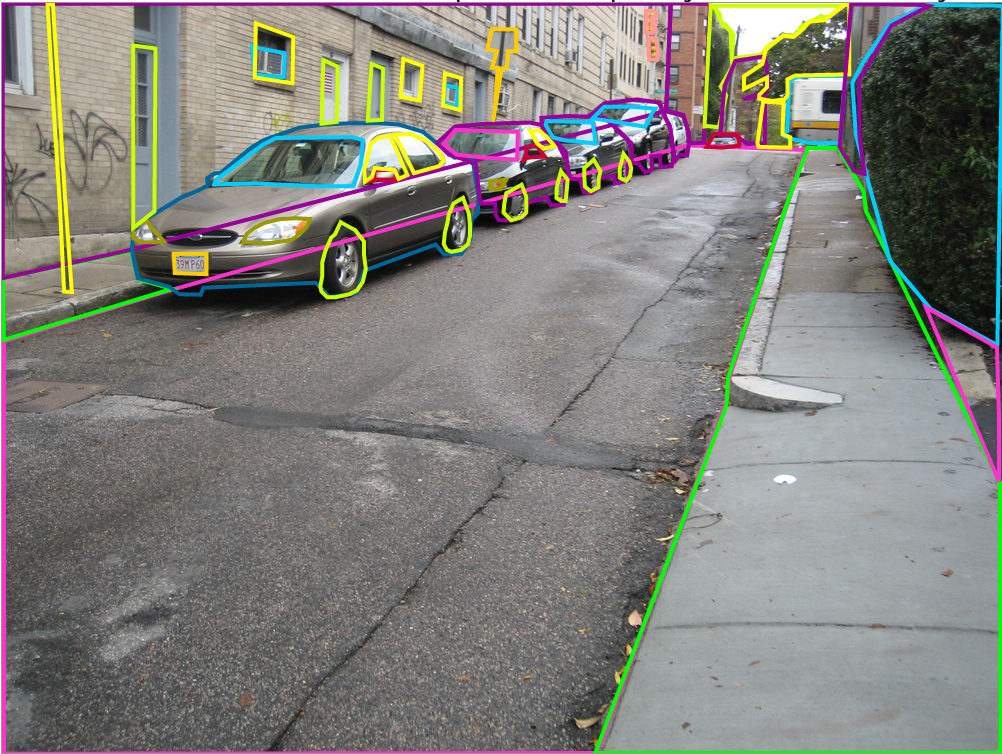
\includegraphics[height=2in]{images/labelmeparse.png}
\caption{An example of a parsed image. Adapted from the website of the
  LabelMe dataset.}
\end{figure*}

 \footnote{cite labelme}

\begin{tabular}{l l}
air conditioning & building\\
bus & car\\
door & headlight\\
license plate & mirror\\
plant & pole\\
road & sidewalk\\
sign & sky\\
traffic light & tree\\
wall & wheel\\
window & windshield\\
\end{tabular}

This is partly motivated by consideration of the human visual system:
\footnote{Pedro suggests Palmer for this whole thing, presumably:

  Palmer, S.E. (1999) Vision Science: Photons to Phenomenology, MIT
  Press .}  
\begin{itemize}
\item Humans use context to resolve ambiguities. \cite{visual-context}
  This means that we can only identify some objects by modeling their
  relationship to other objects. This can be seen in \cite{pop}.
\item Humans interpret some groupings of objects as a larger level
  object or activity, such as crowds of people or flocks of birds.
  Gestalt research demonstrates that perception has definite,
  repeatable grouping rules. \cite{gestalt}
\item Humans seem to interpret whole scenes even when answering
  simpler visual questions, such as edge detection and segmentation.
  This can be seen in Figure \ref{fig-bsd}, which shows an example
  from the Berkeley Segmentation Database. \cite{bsd}
\end{itemize}
\begin{figure}
  \centering
\subfloat[Human Segmentation]{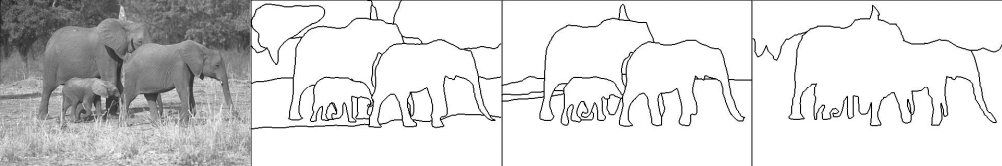
\includegraphics[width=120mm]{images/elephant-human.png}}\\
\subfloat[Machine Segmentation]{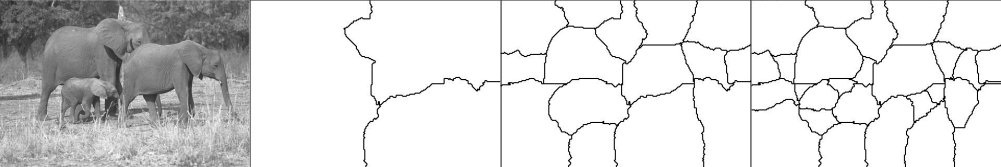
\includegraphics[width=120mm]{images/elephant-machine.png}}
\caption{Even on low-level visual tasks such as segmentation, humans
  give answers based on an interpretation of the whole scene. Figure
  adapted from.}
\label{fig-bsd}
\end{figure}

\footnote{ \cite{bsd}}

Grammatical methods are also motivated by theoretical
considerations. They are a natural choice for modeling large
structural variations (see Section \ref{sec-structural}). Grammatical
models give a principled way to avoid hard decisions for low-level
visual tasks (see Section \ref{sec-soft}). They allow strong models of
background clutter (see Section \ref{sec-clutter}). They allow whole
scene parsing (see Section \ref{sec-whole}). They make it easy to
integrate models from other domains into visual models (see Section
\ref{sec-modules}). Finally, there are theoretical reasons why
grammars may provide better generalization than other models.

\section{Curve Models: An Evolution}

We wish to build probabilistic models of curves, so that we can
calculate a likelihood that a shape class generated a particular
curve. We start by imagining a single input curve, and perturbing it.

The most straightforward model for perturbing a curve is a Markov-type
model. A curve is a sequence of line segments
$\ell_1,\dots,\ell_k$. We can describe the curve by giving the length
$l_i$ of each $\ell_i$, and the angle $\theta_i$ between $\ell_i$ and
$\ell_{i+1}$. If we perturb each $\l_i$ and $\theta_i$ slightly, we
get a curve which differs from the original. Some samples from this
are shown in Figure \ref{fig-markov}.
\begin{figure}
  \centering
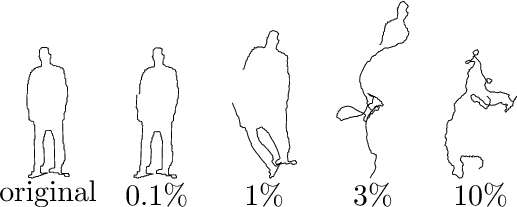
\includegraphics[width=120mm]{images/markov_new.png}
\caption{The problem of drift makes a Markov model unappealing. Random
  samples from this model are too similar locally and too dissimilar
  globally. These shapes were generated by changing each length $l$ by
  a multiplicative factor of $1 + \NNN(0,\sigma)$, and changing each
  angle $\theta$ by adding $\pi \cdot \NNN(0,\sigma )$. Here $\sigma$
  is the value listed underneath the shape.}
\label{fig-markov}
\end{figure}

\begin{figure}
  \centering
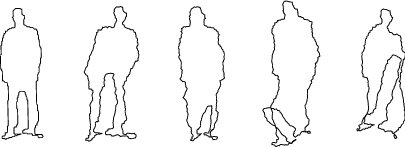
\includegraphics[width=120mm]{images/hcm.png}
\caption{The shape on the left is the original, and the other curves
  have been produced by sampling from the hierarchical curve models of
  . The model produces curves which have more perceptual
  similarity than the Markov model. }
\label{fig-hcm}
\end{figure}
\footnote{\cite{hcm}}

The major weakness of the Markov model is \emph{drift}: the small
errors will accumulate, and the overall shape of the curve will vary
greatly. A straight line has some probability of curling into a tight
spiral. Consider a shape like a hand: a hand has fingers that
protrude. This means that there are two points (namely the two points
where a finger meets the rest of the hand) far away in the curve that
we always expect to be very close together. A Markov perturbation of
the shape is likely to pull these points far apart.

To defeat this problem, \emph{hierarchical curve models} were
introduced in \cite{hcm}. There, the following curve model is given:
\begin{itemize}
\item Given a model curve $C$, decompose $C$ hierarchically by
  repeatedly cutting it in half, in a balanced but otherwise arbitrary
  fashion.
\item Suppose our first decomposition is $C=DE$. We perturb $C$ into
  $C'$ by first perturbing the midpoint of $C$ slightly. We then
  rotate and scale the curves $D$ and $E$ so that $D'$ goes from the
  endpoint of $D$ to the new midpoint, and $E'$ goes from the new
  midpoint to the endpoint of $E$.
\item We then recursively apply the same process to each subcurve $D$
  and $E$. 
\end{itemize}
It is easy to see that this defeats the problem of drift, because the
overall shape of the curve is determined in a constant number of
substitutions from the beginning curve. If our perturbations are
smaller for larger curves, then we will leave the overall shape very
similar while allowing significant local variation. Some samples from
this model are shown in Figure \ref{fig-hcm}.

Hierarchical curve models have room for improvement, as can be seen in
Figure \ref{fig-hcm}. The variations do not respect the perceptual
structure of the original curve; in particular, we do not see
articulated parts being articulated.

In this document, we describe a grammatical reformulation of the work
of \cite{hcm}, which we hope will improve upon it in two
ways. Firstly, we hope to allow for structural variation, which we
argue is an important goal for computer vision in Section
\ref{sec-structural}. Secondly, we give a generative probabilistic model of
curves, which allows us to retrain the parameters of a grammar in a
mathematically sound way, rather than optimizing many parameters in an
expensive and fragile way.

\section{Examples of Grammatical Approaches}

\subsection{Curve Grammars}

We wish to build a model of closed curves in the plane. This is an
important task because curves are the boundaries of objects, and we
can use this fact to recognize some object classes. The shape of a
boundary is invariant to many photometric effects, in particular
illumination. \cite{canny}

\subsection{Visual Chalkboard}

As an example throughout this document, we discuss a system which
would take images of a classroom chalkboard and attempt to parse them
into lecture notes. This is an application with lots of noise. It is
also an application where different levels of interpretation are
required, since lectures can contain both sentences (which should be
interpreted thoroughly, as text) and drawings (which could be
interpreted partially as collections of lines, but which may contain
unsummarizable elements which must be included verbatim).

In Section \ref{sec-modules}, we argue that grammars are a natural
choice for such an application, because they make it possible to
integrate statistical models from other domains in a straightforward
and principled manner.

\subsection{Visual Search Engine}

Google image search is a nice and useful thing, but it relies
partially on images being associated with relevant text on web
pages. It would be nice to find raw or under-described images, and it
would be nice to base search results more on the contents of the
image. We might also submit images as queries, rather than text. The
LabelMe dataset is a good challenge for this task.

In Section \ref{sec-annotation}, we argue that hierarchical
decomposition would allow the necessary rich understanding of
relationships between objects.

\subsection{Other Visual Grammars}
\label{sec-other-grammars}

Many well-performing vision algorithms can be thought of as special
cases of grammatical algorithms. Some examples can be found in
\cite{pop, pictorial, grammar-tr}. Recognizing these as a special case
means that we may be able to improve upon this work by specifying
richer models in some cases, or models that are better mathematically
founded (and thus potentially trainable) in other cases. There are two
tricks for turning a model into a grammar model:
\begin{itemize}
\item Mixture models are a special case of grammar models. If we have
  mixture components $M_1,\dots,M_k$ with mixture weights
  $p_1,\dots,p_k$, then we can build a grammar model $M$ in which we
  have rules:
  \begin{align*}
    M &\to M_1 &(p_1)\\
     &\to M_2 &(p_2)\\
     &\dots&\\
     &\to M_k &(p_k)\\
  \end{align*}
  The same is true of nearest neighbor models. This is exciting
  because mixture models and nearest neighbor models are often very
  powerful, but do not generalize well from a small amount of data.

\item Deformable parts-based models are a special case of grammar
  models. Let $M(x)$ denote the hypothesis that model $M$ appears at
  image location $x$. If we have part models $P_1,\dots,P_k$, then we
  can build a grammar model $M$ which has the rules:
  \begin{align*}
M(x) &\to P_1(x + \delta_1) + \dots + P_k(x + \delta_k)\\
P_i(x) &\to P_i(x+\Delta)\\
P_i(x) &\to I(x_1 \pm w_i, x_2 \pm h_i)
  \end{align*}
  The $\delta_i$ represent the ideal displacement of each part $P_i$
  from the object model. The model is deformable because the second
  kind of rule allows the parts to be randomly displaced. The
  probability of $P_i(x) \to P_i(x+\Delta)$ will depend on
  $\Delta$. The third kind of rule gives the cost to place a part,
  which can be thought of as the negative log probability that a part
  $P_i$ would produce the image data under it, $I(x_1\pm w_i, x_2\pm
  h_i)$.

  In our model of curve grammars, the second kind of rule is given
  by the midpoint distribution $\mu_{X\to YZ}$, and the third kind of
  rule is trivial (see Section \ref{sec-pcfsg}).
\end{itemize}

\section{Grammatical Vision is Important}

\section{Hierarchical Decomposition and Rich Description}
\label{sec-annotation}

It would be very useful if vision algorithms could achieve richer
understanding of scenes, and produce richer descriptions of images. A
rich understanding of a scene requires an understanding of the
relationship between objects. Consider an image containing a person
and two objects, where the person is pointing at one of the
objects. This is an important piece of information, and it cannot
easily be described by a list of the objects in the image.

Some scenes contain important objects that are nothing more than a
particular grouping of other objects: a crowd is just a collection of
people. Moreover, the nature of the collective object is determined
partly by the relationship between its elements. A crowd and a
marching band are two very different objects, but this difference
cannot be expressed in a simple listing of objects. How can vision
algorithms achieve this level of understanding, or even represent it?

One straightforward and general framework for rich description is a
labeled hierarchical decomposition of a
scene. \cite{zhu-mumford} This takes the form of a tree, where:
\bitem
\item The root node describes the entire image.
\item Each node is labeled with the name of an object, and an area of the image described. These areas may be approximate.
\item The children of a node describe sub-parts of the parent, and
  have areas inside the parent node's area.
\eitem
We can explicitly encode such a description in an XML-like language.
Since grammatical methods produce and work with such hierarchical
decompositions, they give a natural model for such structures.

In the example of the visual chalkboard, rich description would
produce more useful output than simple text. For instance, in
transcribing a series of boards as lecture notes, we would like to be
able to label non-textual regions as figures and include them
verbatim, or render them as a collection of lines.

\subsection{Training on rich annotations}

We would also like to train grammars simultaneously on an image and a
hand-made rich hierarchical description of that image. This ensures
that our trained grammars will produce semantically meaningful
decompositions of new images: the decomposition will have a structure
similar to that produced by a human, and we will be able to transfer
labels onto the nodes of the decomposition.

This will make it more feasible to output meaningful rich descriptions
on a wide range of data. Stochastic grammatical methods allow us to
put soft constraints on descriptions (``it is unlikely that a person
will have an apple for a face''), which will be more flexible and less
brittle than hard constraints (``a person's face can have eyes, nose,
etc., but not fruit''). We can thus favor more realistic descriptions
of scenes while still producing useful output on very unrealistic
scenes (such as Magritte's ``The Son of Man'').

Note that we may still gain information from rich descriptions without
a specified correspondence to particular parts of the image. Knowing
the correct structure and guessing at the exact correspondence is no
harder than guessing both the correct structure and the
correspondence. Such descriptions would be less labor-intensive to
produce, so we might be able to train on larger datasets.

In general, supervised learning is easier than unsupervised
learning. In computational linguistics, this means that learning a
grammar for natural language is much more tractable given samples of
natural language that have been parsed. (These are called
\emph{bracketed samples}.) It is likely that training on rich
annotations would also make learning visual grammars much easier.

\subsection{Some Problems with Rich Description, and Solutions}

For a number of reasons, dealing with rich descriptions is more
complicated than dealing with simpler descriptions. Grammatical
methods and hierarchical decomposition give ways around some of these
problems. Some important issues are: Class/Subclass ambiguity
and Questionable Parts.

First, it is worth noting that hierarchical decomposition degrades
gracefully into a flat description, since we can always decompose the
root node into a list of objects. Hierarchical decomposition presses,
but does not force, us to explain how any two parts of our annotation
are related, making for more useful description.

\bitem

\item Decomposition provides a reasonable and elegant solution to the
  Questionable Parts problem. David Marr explained it thus:
  \begin{quote}


    % What, for example, is an object, and what makes it so special that
    % it should be recoverable as a region in an image?

    Is a nose an object? Is a head one?  Is it still one if it is
    attached to a body?  What about a man on horseback?

    These questions show that the difficulties in trying to formulate
    what should be [considered an object] %recovered as a region from
                                %an image 
    are so great as to amount to philosophical problems.  There really
    is no answer to them - all these things can be an object if you
    want to think of them that way, or they can be a part of a larger
    object...% (a fact that is captured quite precisely in Chapter 5).
    \cite{marr}
  \end{quote}

  In any annotation system rich enough that we might simultaneously
  label a wheel and a car, or eyes and a face, in the same image,
  there is an arbitrary choice of how many things to label. Forcing
  these descriptions to be consistent is very
  difficult. \cite{labelme} This is especially pronounced with
  agglomerations, like crowds of people. There is no point at which a
  group of people meaningfully becomes a ``crowd''; two people are not
  considered a crowd, and one hundred people are considered a crowd,
  but it is impossible to draw a clear line between crowds and
  not-crowds.

Forcing consistency may even be counter-productive. If we must label
every face in a crowd, then a crowd seen from a distance will have an
enormous number of face labels, most of which are basically
guesses. If we never label faces in a crowd, then our visual search
engine may fail to retrieve images of a particular person when they
are in a group, even if they are clearly visible. 
  
Hierarchical decomposition describes a scene as a hierarchy of
objects, and further decomposition of these objects is optional; as
long as we know something about the object's appearance, we don't have
to demand that it be broken up into its constituent parts.

\item Grammatical methods also naturally address the Class/Subclass
  Ambiguity problem: descriptions of an object can be general or
  specific, and the level of specificity is fairly arbitrary. It is
  clear that we want the query ``dancer'' in a visual search engine to
  return images of people dancing, but these same images should also
  be returned on the query ``person''. 

  Grammatical methods model such ambiguity as OR nodes in an AND-OR
  structure \cite{zhu-mumford}, or by rules of the form
\begin{align*}
\mathrm{CLASS} &\to \mathrm{SUBCLASS}_1\\
&\to \dots\\
&\to \mathrm{SUBCLASS}_k .\\
\end{align*}

The LabelMe dataset uses a set of labels derived from WordNet
\cite{wordnet} that are related via class-subclass
relationships. The maintainers of the dataset claim that it requires
very little work to map the arbitrary labels provided by users into
these more precise and formalized labels. \cite{labelme} Given
such techniques, the Class-Subclass ambiguity problem is probably not
a fundamental barrier to rich description.

\eitem

\subsection{Rich Description and XML}

The rich descriptions we have described are naturally represented in
XML and similar languages, which yields some opportunities: 

\begin{itemize}
\item XML is reasonably human-readable and human-writable. (Comparable
  formats like YAML are even more so.) This means that rich
  photo-tagging could be done by many people, and also that many users
  could benefit from a visual search engine that accepts structured
  queries. For example, photos inside of an image could be recursively
  described as such, allowing us to separate the images containing an
  actual movie star from those containing a poster depicting that
  movie star. As another example, having a notion of classes and
  subclasses would allow us to search for \texttt{BASS < FISH} and
  receive only pictures of bass fish, and not pictures of the
  instrument or of other fish.

\item Existing technology such as XPath allows computer programs to do
  efficient and flexible searches on XML documents. This means that
  fairly complex image-sorting tasks could potentially be automated.
  This could be very good, because some image-sorting tasks such as
  content moderation are reported to be very psychologically
  damaging when performed by humans.

\item One particular XML-based file format is the \emph{scalable
    vector graphics} format (SVG). If we can learn rich visual
  grammars, we could hope to recover artistic information from images,
  so that we could approximate a drawing as a collection of strokes in
  fills in an SVG document.

  Ultimately, we might hope to learn artistic concepts such as drawing
  style or font, which would greatly expand the power of graphics
  programs.
\end{itemize}

\section{Grammars and Statistical Models}

\subsection{Structural Variation}
\label{sec-structural}

Natural object categories such as cars and people exhibit two kinds of
variation: small deformations and large structural
variation. Therefore, object models which allow for both will make
vision algorithms much more powerful.  The potential for a satisfying
account of large structural variation is one of the most intriguing
possibilities of grammatical methods.

One of the simplest structural variations is occlusion: part of an
object may not be visible, usually because something between the
object and the camera is occluding it. Occlusion has been well
understood in computer vision for a long time, and models can be made
robust to it, e.g., the Hausdorff distance in \cite{hausdorff}. 

Another common way that objects exhibit structural variation is by
having \emph{optional parts}: a dog may or may not have a tail, a
person may or may not have a hat. Occlusion models are capable of
recognizing such objects with or without their optional parts, but
they do not accurately model optional parts. An optional part is a
particular subset of the object that is likely to not appear, while
occlusion allows any not-too-large subset of the model to disappear.

The usefulness of more general structural variation can be seen in
Figure \ref{fig-variation}. Here, the human eye notices a large
similarity between the two shapes $A_1$ and $A_2$, but many curve
models would see very little similarity.

\begin{figure}
  \centering
\subfloat[$A_1$]{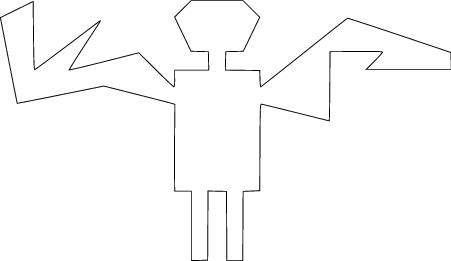
\includegraphics[height=30mm]{images/basri_original.png}}
\subfloat[$A_2$]{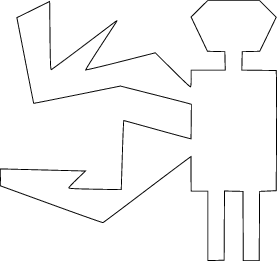
\includegraphics[height=30mm]{images/basri_variation.png}}\\
\subfloat[$A_3$]{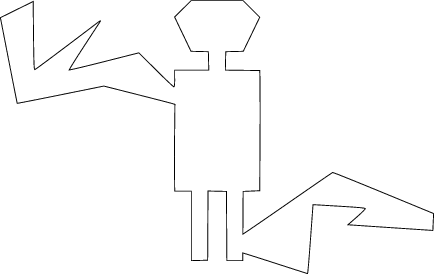
\includegraphics[height=30mm]{images/basri_variation_bad2.png}}
\subfloat[$A_4$]{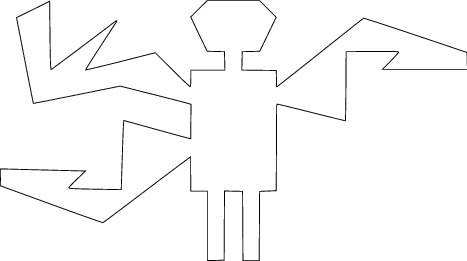
\includegraphics[height=30mm]{images/basri_three.png}}
\caption{If $A_1$ is the original curve, which other curve is most
  similar to it? Figure adapted from .}
\label{fig-variation}
\end{figure}
\footnote{\cite{basri-jacobs}}

We might intuitively describe the second shape, $A_2$, as
$$ A_2 =\mbox{``Take $A_1$, snap off the right appendage, and reattach
  it beneath the left appendage.''}. \label{desc-variation}$$ 
This highlights several important points:

The description \ref{desc-variation} of $A_2$ is very short in
English, and might be even shorter in a specialized curve model
encoding. Description length is a good proxy for the conditional
probability of observing $A_2$ given that it is a distortion of $A_1$
\cite{potter-geman-bienenstock}.

Structural variation is a fundamental problem in modeling visual
objects. In the absence of a practical model of structural variation,
we must model variation as continuous deformation. Then, any model
that declares $A_1$ and $A_2$ to be similar will think that $A_3$ or
$A_4$ is even more similar to $A_1$.

Structural variation cannot be modeled without a semantically
meaningful decomposition of the original curve, like that seen in
Figure \ref{fig-variation-decompose}. Description \ref{desc-variation}
crucially relies on ``the right appendage'' making sense to the
listener. Thus, perceptually simple structural variation must respect
the perceived structure of the original curve. Contrast Figure
\ref{fig-variation} with Figure \ref{fig-badvariation}, where a
similar transformation has been applied with no regard to the
perceived structure of the original curve.

\begin{figure}[h]
\centering
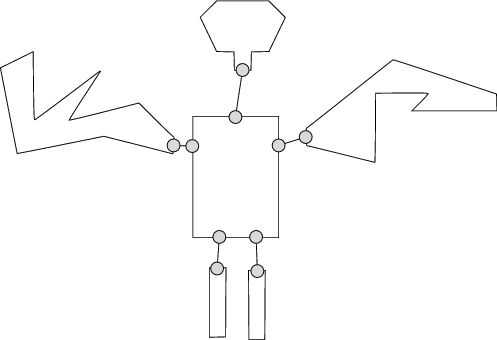
\includegraphics[height=30mm]{images/basri_decomposed.png} 
\caption{The original shape from Figure \ref{fig-variation},
  decomposed into semantically meaningful parts. We argue that this
  decomposition explains why the variation in Figure
  \ref{fig-variation} is less semantically different than the
  variation in Figure \ref{fig-badvariation}. Adapted from
.}
\label{fig-variation-decompose}
\end{figure}
\footnote{\cite{basri-jacobs}}

\begin{figure}[h]
\centering
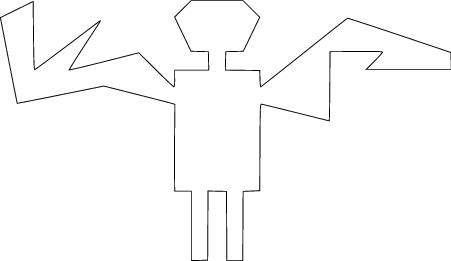
\includegraphics[height=30mm]{images/basri_original.png} 
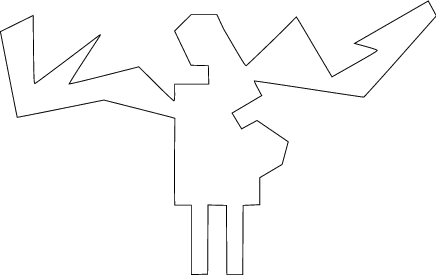
\includegraphics[height=30mm]{images/basri_variation_bad.png} 
\caption{Two shapes which are not perceptually very similar, although
  they are related by a transformation as simple as that in Figure
  \ref{fig-variation}. The problem is that the transformation does not
  respect the perceived structure of the original. Adapted from
  .}
\label{fig-badvariation}
\end{figure}
\footnote{\cite{basri-jacobs}}

Mixture models are a class of models that do not suffer from the
continuous deformation problem of Figure \ref{fig-variation}. However,
if there are multiple independent structural variations possible, it
is unlikely that we will see every combination of each form.  Consider
the shape grammar $\GGG_n$ that generates shapes that have $n$ arms,
each of which can take either of two forms:
\begin{align*}
S&\to \underbrace{Z\dots Z}\\
&\phantom{\to Z ..}n\\
Z &\to A\\
Z &\to B,
\end{align*}
where $A$ is pointy and $B$ is rectangular. We show four shapes
possible under this grammar in Figure \ref{fig-narms}. 
\marginnote{Change these to outline instead of solid shapes!}
\begin{figure}[h]
\centering

\includegraphics[height=30mm]{images/narms.png} 
\caption{Four shapes from $\GGG_8$.}
\label{fig-narms}
\end{figure}
A classic mixture model will not be able to generalize in this
scenario without exponentially many training examples, since there
are $2^n$ possible shapes. If we instead have mixture models at the
level of individual structural variations, then our model is a
grammatical model in the style of Section \ref{sec-other-grammars}.


\subsection{Soft Decisions}
\label{sec-soft}

While human vision crucially relies on global context to resolve local
ambiguity \cite{visual-context}, computer vision algorithms often have
a pipeline which makes hard low-level decisions about image
interpretation, and then uses this output as input to higher-level
analysis. Algorithms will be more accurate and less brittle if they
can avoid making such hard decisions, as advocated in \cite{pop,
  jin-geman}.

For example, in the visual chalkboard, there will be various stray
marks on the chalkboard. We would prefer not to filter these out with
some sort of quality threshold, but instead mark them as
possibilities, try to assemble an overall interpretation of the board,
and then discount any stray marks that do not participate in the
interpretation. This seems much more fruitful than filtering out stray
marks, along with some genuine letters, and then having to be very
forgiving of words actually missing some of their letters altogether.

This requires us to combine and resolve information at different
levels. Grammatical methods provide us with powerful inference
algorithms for determining the most likely decomposition of a scene
under a given compositional model. Since important local ambiguities
will lead to different global decompositions, this is exactly what is
needed: the overall likelihood of the decomposition is a common
currency that allows us to negotiate between fitting the local data
well, and explaining the local data in a way that allows a good
decomposition of the rest of the image.

\subsection{Modeling Clutter with Object Sub-parts}
\label{sec-clutter}

We would like to build specific and accurate models of clutter.  For
instance, for the visual chalkboard, it would be helpful to have a
model for stray chalk marks, rather than a model for arbitrary
unexplained patches; otherwise we will be tempted to explain stray
chalk marks as some letter, possibly a lower-case 'i'. If we try to
set our threshold high enough that we don't do this, we might start
labeling some genuine i's as background. If we instead have a model
for chalk marks, we can explain stray chalk marks and i's as
particular sorts of chalk marks, and differentiate them based on
context and appearance.

\cite{jin-geman} suggests modeling clutter in the background with
sub-parts of the objects of interest. Since objects in the background
are still objects, and are often related to the objects of interest,
this might allow us to build a much stronger background model in many
cases. In addition, by modeling clutter with sub-parts, we are less
likely to hallucinate whole objects when we see sub-parts. Thus, it is
especially important that we have a cheap way to explain clutter that
closely resembles sub-parts of the objects of interest.

With such a system, we might even be able to ignore rather subtle
clutter, such as some stray letters, or even words, from a previous
lecture that was not completely erased. Clutter words would not be
part of a line of text, and would thus be identifiable as clutter in
the parsed output, where they would be excluded from the main body of
text.

\subsection{Whole Scene Parsing}
\label{sec-whole}

It is useful to demand whole scene parses, since it avoids the need to
fine-tune detection thresholds and decision boundaries
\cite{pop}. Consider the example of the visual chalkboard. Instead of
having to set a filter on chalk marks to filter out stray chalk marks,
we simply explain them and discount them, since they are not part of
any larger structure, such as a word, that we find interesting.

\subsection{Statistical Modules}
\label{sec-modules}

Grammatical methods offer a very powerful and general way to make
vision algorithms more robust: if we can integrate different
statistical models in a modular fashion, especially models trained in
different contexts, then our system will be more robust than any
single model.

Grammatical methods are well-suited to integrating any statistical
model that depends on the qualities of image objects and the
relationships between them. When we can map objects and relationships
between domains (for example, mapping pictures of text to actual
text), this allows us to import already-trained statistical models
from very different domains.

Consider transcribing a lecture from the visual chalkboard. The system
will better recover from misidentifying letters if it uses
higher-level knowledge about the lecture's language and contents. In
particular, we can build a single grammar that integrates such
tried-and-true models as the $n$-gram model of letters
\cite{manning-schutze}, the $n$-gram model of words
\cite{manning-schutze}, a stochastic grammar model of phrase and
sentence structure \cite{manning-schutze}, and topic models of word
choice in the subject of the lecture \cite{lda}. All of these models
can be trained on large corpora of text, rather than on smaller
datasets of images.

% Each of these models can easily be expressed in a grammatical way,
% since each gives a likelihood that can be written as a product over a
% decompositional tree structure: 
% \bitem
% \item The $n$-gram models can be written as a product over any tree
%   that respects the linear order of the letters or words. Each factor
%   judges the likelihood of the $n$-grams that bridge the two
%   subtrees.
% \item The stochastic grammar model is itself a grammar, and the
%   trees are the same.
% \item The topic model can simply penalize the nodes corresponding to
%   words according to how common each word is.
% \eitem

% Grammatical methods can potentially express rich relationships between
% model parts through the formation probabilities $\Phi_{M\to P_1\dots
%   P_k}$ considered in Section \ref{sec-other-grammars}.

\subsection{Independence and the Poverty of Stimulus}

Grammatical models are typically context-free, which is fundamentally
about making independence assumptions. We argue that independence
assumptions can increase the effective amount of training data you
have.

\begin{rem}[Context-freeness is an independence assumption]
Grammatical methods in general are characterized by 1) a method for
decomposing novel data in a hierarchical fashion, and 2) an
explanation for each level of the hierarchy in terms of previously
seen data. For example, in a standard CFG, we will have both a parse
tree over a sentence, and a set of labels for the nodes of the parse
tree. If the CFG has been automatically generated (i.e., no human has
assigned semantic meaning to grammar elements), then the set of labels
for the nodes is just a probability distribution derived from all
parts of the training set that have received the same label. 

For generic grammatical methods, we can assume context-freeness by
specifying that the contents of a node N (all nodes below N in the
hierarchy) are independent of the context in which N appears (all
nodes not below N in the hierarchy) given the data stored at N (its
label and any attributes).
\end{rem}

\begin{rem}[Independence assumptions yield more effective data]
  Independence assumptions let you effectively multiply the amount of
  data you have. Consider the following simple problem: try to
  classify 0-1 vectors into two classes given a bunch of labeled
  examples. Consider the two sort of extreme things we can do: if we
  assume that each coordinate of the vector is independent, we get a
  Naive Bayes classifier, where we basically learn what the
  distribution is over a given coordinate for each class. This can be
  done with a small number of training examples.

  The other extreme is assuming that there is total dependence, that
  there is no relation between any two vectors. Then the maximum
  likelihood classifier (Paranoid Bayes?) is given by seeing how many
  times a specific vector showed up in each class, and picking the
  class where it showed up more often. We would have to guess on any
  novel vector.  

  If the independence assumption is valid for the data, then the Naive
  Bayes classifier acts like the Paranoid Bayes classifier trained on
  a data set that is exponentially larger. (Specifically, for each
  class, we generate all possible vectors that can be made by taking
  the first coordinate of a random example from the class, then taking
  the second coordinate from an independently chosen random example
  from the class, etc.)
\end{rem}

Even when the independence assumption does not apply, context-free grammars
are useful. This can be seen in examining the classic nonsense
sentence "Colorless green ideas sleep furiously". The supposed
weakness of context-free grammars, that the context-free assumption is
unrealistic, is actually a strength, because it allows us to parse and
react to very unrealistic data.

% \section{Computational Considerations}

% \subsection{Bidirectional Pipeline}
% \note{ {\bf (write!, sources)}}

% If we avoid hard decisions whenever possible, our algorithms must sift
% through a larger number of intermediate hypotheses. This can be made
% more efficient by doing a form of data-driven parsing that combines
% the strengths of top-down and bottom-up parsing. One example of this
% approach is given in \cite{astar}.

% \subsection{Sharing Object Parts for an Enormous Object Dictionary}
% \label{sec-shared}

% \note{  {\bf (write!)}}

% \note{Not true that it is impractical! Systems exist! Just say it is difficult, I guess. Should we cite the systems?}
% It is currently impractical for vision systems to know about more than
% a certain number of object classes, something like several hundred for
% adequate performance. It would be very useful if we could increase
% this number, so that we have a vision system capable of dealing with
% tens of thousands of object classes.

% This is impractical unless we can devise algorithms which are
% sublinear in the number of known object classes. This, in turn,
% requires that our set of models admits some sort of search
% structure.

% Some work has been done on hashing image patches.
% \note{find}

% By composing a small set of parts which are very distinguishable, we
% will have an exponentially large number of models. Otherwise, the hash
% table just fills up and we have to go through a bunch of false positives.

% \note{ About 30000 entry-level object categories \cite{biederman}}

% \note{Even with a reasonably small set of parts, we still need to be
%   able to search without enumerating models. This could be something
%   like a k-d tree or a hash function. \cite{biederman}}

% For the visual chalkboard, the letters of the alphabet would form a
% small set of parts that combine to produce many objects, potentially
% any word in a very large dictionary.

\section{Grammatical Vision is Difficult}

Little concrete progress has been made with visual grammars. The
general frameworks have few practical results, and people with
practical results don't seem to have a general framework.  \marginnote{This
  statement feels too strong. But something like this has to be said.}

We are also hindered because the closest equivalent to linguistics is
the cognitive science of vision, which is not as well-stocked with
intermediate hypotheses and sanity checks. For example, in
linguistics, utterances can be decomposed into phonemes. There is no
agreement as to how a visual signal can be decomposed.

\section{Grammar induction is difficult}
\label{sec-gram-hard}

Grammatical methods in vision are inspired by grammatical models like
probabilistic context-free grammars in linguistics. In computation
linguistics, the problem of learning a grammar from unlabeled examples
(grammar induction) is very difficult.

There are many \cite{lee-induction} negative theoretical results, the
most fundamental of them being Gold's Theorem:

\begin{thm}[Gold's Theorem]
Consider an algorithm $A$ trying to learn a language $L\in \Sigma^*$.
$A$ is given an infinite sequence of words $w_1, w_2, \dots\in L$ which
contains every word in $L$ at least once. After each $w_i$, $A$
outputs some $L_i$. $A$ is said to {\em learn $L$ in the limit} if,
for some $n$, $L = L_n = L_{n+1} = L_{n+2} = \dots$.

Then, if a class of languages $\LLL$ contains all languages of
finitely many strings, and at least one infinite language (in
particular, if $\LLL$ is the set of context-free languages), no
algorithm can learn all languages in $\LLL$ in the limit.
\end{thm}
Note that this result applies to all algorithms, regardless of their
complexity. 

This is a fundamental theoretical barrier to grammar induction. There
is some hope that we can defeat it by adopting a Bayesian approach,
and only hoping to learn sufficiently simple grammars. This has been
attempted several times, but no solution is known for the associated
Bayesian learning problem, and a heuristic search strategy must be
used \cite{cook, stolcke, nevill-manning}.

It is clear that the problem of learning context-free grammars applies
directly to curve grammars, since part of our curve model actually is
a PCFG (see Section \ref{sec-pcfsg}). The learning problem might be
easier if visual grammars can be simpler in structure than string
grammars for natural languages. We don't know if this is the case.

\section{Visual Grammars are hard for additional reasons}

\subsection{Comparisons are Always Inexact}

The continuous nature of visual signals means that we will rarely if
ever see exact agreement between two visual objects at the pixel
level. Compare a well-defined linguistic object (such as a word) to a
visual part such as an eye; an eye will look slightly different in
every image because of natural variation and photometric
effects. Because language has predefined symbols, in the case of
written language, or agreed-upon phonemes, in the case of spoken
language, methods from computational linguistics can check whether two
letters or two words are the same. Working with visual grammars is
thus analogous to trying to solve the problems of computational
linguistics simultaneously with the problems of speech recognition.

Computational linguistics algorithms can also be given hand-labeled
information about pre-existing correspondences between samples. For
example, there are datasets of sentences which come with ground-truth
grammatical parses. Such information is generally unavailable in
vision. 

Without certain knowledge of correspondence between samples,
generalization is difficult. We are required to infer correspondences
between samples in an unsupervised manner. This generally leads to a
unsupervised learning problem, such as clustering, or a correspondence
problem.

\subsection{Dealing with Scale}

Computer vision usually tries to be scale invariant, since a small
object closer to the camera naturally looks like a large object
further from the camera. A doubled copy of an image is hopefully
semantically the same as the original image.

We thus have two problems: when an object is too small, its internal
structure may be lost. Generally, fine internal structural elements
first become texture (discernible en masse but not individually) and
then disappear completely. The larger object may still, however, be
recognizable by shape.

When an object is too large, we are faced with the task of parsing
internal structure of which we were previously unaware.

These difficulties can probably be dealt with. The first demands that
we come up with a simple appearance model for every object, so that we
can detect it without detecting any of its subparts. Decreased recall
is probably OK, as smaller things are actually more difficult to see.

The second demands that every object be detectable at large scales,
even those which have no sub-parts in our grammar. We can model this
with simple infinitely recursive grammars; sufficiently simple ones
can hopefully model almost anything, while basically preventing their
being bias for either one of: 
\bitem
\item A ``larger'' model with more internal structure
\item A ``smaller'' model with less internal structure
\eitem

\subsection{Plane grammars do not naturally admit efficient parsing}

Efficient algorithms for parsing strings with context-free grammars
rely on dynamic programming, and ultimately on the fact that a string
has only quadratically many contiguous substrings. The elements of
visual grammars naturally live in the image plane, and thus do not
have a linear order. A visual object need not even occupy a single
contiguous region, in the case of occlusion. Therefore, a parsing
algorithm might in principle have to consider any subset of the image
elements as a node in the parse, leading to an exponential runtime.

There are some ways to address this problem.

% \section{Prior Work and Literature Review }
% \note{{\bf (write!)}}

% \bitem
% \item Visual Grammars:
% \bitem
% \item Stu Geman and Ya Jin's work
% \item visual L-systems
% \eitem
% \item Grammar Induction:
% \bitem
% \item \cite{stolcke}
% \item Dan Klein 
% \item \cite{charniak}
% \eitem
% \eitem

\marginnote{beginning of intro.tex}
